\chapter{Results}
\label{ch:results}

All scores come from the official validation splits. WEMoE rows give the mean and standard deviation over seeds 0, 1 and 2.

\section{Results by Task}

Table~\ref{tab:per-task} and Figure~\ref{fig:per-task} give the scores per task, and Table~\ref{tab:gain} places each merged model between the majority class and the expert. The experts themselves are not equally strong. SST-2 and QNLI, with the most training data, score above 90. RTE scores only 63.2, and its dev score was still rising at the last epoch (49.0, 65.5, 65.9). Expert training took 43 minutes in total: 0.8, 0.7, 1.1, 11.0 and 29.8 minutes for MRPC, RTE, CoLA, SST-2 and QNLI, with best epochs 2, 3, 3, 2 and 3.

\begin{table}[htbp]
  \centering\tablestyle
  \caption{Per-task scores ($\times100$). Bold marks the WEMoE $k=256$ results that fall below the majority class.}
  \label{tab:per-task}
  \setlength{\tabcolsep}{3pt}\begin{tabular}{l c c c c c}
    \toprule
    Model & MRPC (Acc/F1) & RTE (Acc) & CoLA (MCC) & SST-2 (Acc) & QNLI (Acc)\\
    \midrule
    Majority class & 68.4 / 81.2 & 52.7 & 0.0 & 50.9 & 50.5\\
    Simple Averaging & 68.4 / 81.2 & 46.9 & 23.3 & 55.4 & 65.9\\
    Task Arithmetic & 68.6 / 81.3 & 47.3 & 16.9 & 69.8 & 77.9\\
    Input-independent, $k$=256 & 68.4 / 81.2 & 47.3 & 20.2$\pm$0.0 & 70.9$\pm$0.1 & 78.6$\pm$0.0\\
    WEMoE full, $k$=16 & 68.7$\pm$2.3 / 80.6$\pm$2.2 & 48.0$\pm$1.0 & 27.6$\pm$14.1 & 79.6$\pm$8.1 & 74.0$\pm$6.5\\
    WEMoE full, $k$=64 & 71.6$\pm$4.4 / 80.9$\pm$4.3 & 54.0$\pm$3.4 & 20.5$\pm$17.8 & 89.0$\pm$0.6 & 83.1$\pm$2.4\\
    WEMoE full, $k$=256 & 76.3$\pm$4.5 / 83.9$\pm$2.8 & \textbf{52.0$\pm$4.4} & 42.6$\pm$0.9 & 88.0$\pm$0.5 & 86.7$\pm$0.7\\
    WEMoE intermediate, $k$=256 & \textbf{66.5$\pm$0.7 / 76.6$\pm$1.0} & 59.0$\pm$0.9 & 41.7$\pm$0.9 & 86.7$\pm$0.2 & 86.5$\pm$0.2\\
    Single-task experts & 82.1 / 88.1 & 63.2 & 59.1 & 92.2 & 91.2\\
    \bottomrule
  \end{tabular}
\end{table}

\begin{figure}[htbp]
  \centering
  % Palette: reference categorical order validated with the dataviz validator (contrast WARN is relieved by the
% marker shapes, the legend and Table~\ref{tab:main}).
\definecolor{sA}{HTML}{2A78D6}\definecolor{sB}{HTML}{EB6834}\definecolor{sC}{HTML}{1BAF7A}
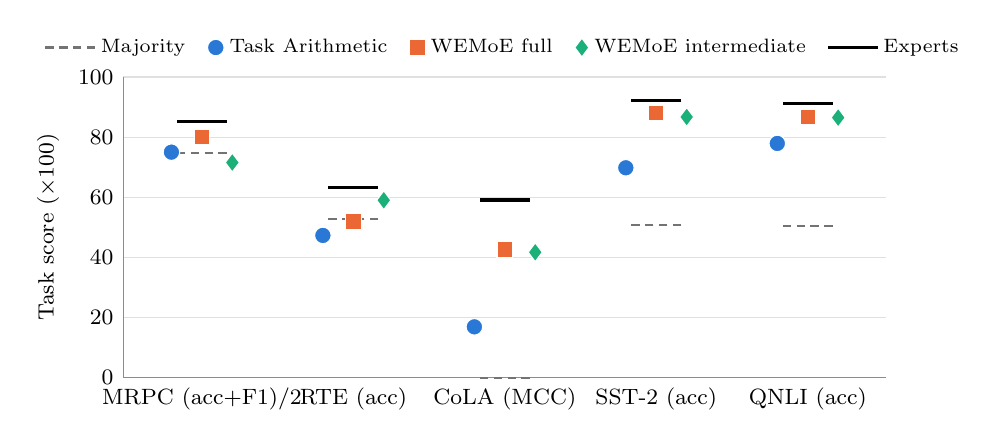
\begin{tikzpicture}
\begin{axis}[
  width=.93\linewidth, height=5.4cm,
  symbolic x coords={MRPC,RTE,CoLA,SST-2,QNLI}, xtick=data, enlarge x limits=.13,
  xticklabels={{MRPC (acc+F1)/2},{RTE (acc)},{CoLA (MCC)},{SST-2 (acc)},{QNLI (acc)}},
  ymin=0, ymax=100, ytick={0,20,40,60,80,100}, ylabel={Task score ($\times100$)},
  ymajorgrids, grid style={black!12}, axis line style={black!45}, tick style={draw=none},
  tick label style={font=\footnotesize}, label style={font=\footnotesize},
  clip=false, axis x line*=bottom, axis y line*=left,
  legend style={at={(.5,1.03)},anchor=south,legend columns=5,draw=none,font=\scriptsize,/tikz/every even column/.append style={column sep=6pt}},
]
\addplot[only marks,mark=-,mark size=9pt,thick,black!55,densely dashed] coordinates {(MRPC,74.8) (RTE,52.7) (CoLA,0) (SST-2,50.9) (QNLI,50.5)};
\addlegendentry{Majority}
\addplot[only marks,mark=*,mark size=3pt,sA,mark options={fill=sA,draw=white},xshift=-11pt] coordinates {(MRPC,75.0) (RTE,47.3) (CoLA,16.9) (SST-2,69.8) (QNLI,77.9)};
\addlegendentry{Task Arithmetic}
\addplot[only marks,mark=square*,mark size=2.8pt,sB,mark options={fill=sB,draw=white}] coordinates {(MRPC,80.1) (RTE,52.0) (CoLA,42.6) (SST-2,88.0) (QNLI,86.7)};
\addlegendentry{WEMoE full}
\addplot[only marks,mark=diamond*,mark size=3.4pt,sC,mark options={fill=sC,draw=white},xshift=11pt] coordinates {(MRPC,71.55) (RTE,59.0) (CoLA,41.7) (SST-2,86.7) (QNLI,86.5)};
\addlegendentry{WEMoE intermediate}
\addplot[only marks,mark=-,mark size=9pt,very thick,black] coordinates {(MRPC,85.1) (RTE,63.2) (CoLA,59.1) (SST-2,92.2) (QNLI,91.2)};
\addlegendentry{Experts}
\end{axis}
\end{tikzpicture}

  \caption{Task scores of the merged models between the majority class (dashed tick) and the experts (solid tick). WEMoE values use $k=256$ and are means over three seeds.}
  \label{fig:per-task}
\end{figure}

\begin{table}[htbp]
  \centering\tablestyle
  \caption{Gain over majority per task, in percent, computed from the seed means.}
  \label{tab:gain}
  \begin{tabular}{l r r r r r r}
    \toprule
    Model & MRPC & RTE & CoLA & SST-2 & QNLI & Mean\\
    \midrule
    Task Arithmetic & 1.8 & $-51.7$ & 28.6 & 45.8 & 67.3 & 18.4\\
    Input-independent, $k=256$ & 0.0 & $-51.7$ & 34.2 & 48.5 & 68.9 & 20.0\\
    WEMoE full, $k=256$ & 51.5 & $-6.9$ & 72.2 & 89.7 & 88.9 & 59.1\\
    WEMoE intermediate, $k=256$ & $-31.6$ & 59.8 & 70.5 & 86.8 & 88.5 & 54.8\\
    \bottomrule
  \end{tabular}
\end{table}

The average improvement does not apply uniformly. On SST-2 and QNLI, the trained routers recover close to 90\% of the gain, and on CoLA about 70\%, against 45.8, 67.3 and 28.6 for Task Arithmetic. Static merging is close to a constant prediction on the two smallest tasks. Its RTE accuracy of 47.3 equals 131/277, the share of the \emph{minority} class, which is consistent with one label for every example, and its MRPC scores barely differ from the majority class. WEMoE does not fully repair this. The full-MLP model recovers about half of the gain on MRPC but does not reliably beat the majority class on RTE: its three seeds give 49.5, 57.0 and 49.5, against 52.7. The intermediate-only model recovers 59.8\% on RTE but falls below the majority class on MRPC. No merged model matches an expert on any task.

\section{Comparison with Relevant Baselines}

Table~\ref{tab:main} gives the aggregate comparison. Task Arithmetic reaches 57.4 and recovers only 18.4\% of the gain, although its normalised score of 70.6 would suggest much more. Before training, the full-MLP model is close to it ($57.8\pm0.6$) but not identical, because the small random router weights move CoLA in particular. At $k=256$, FSFT raises the model to $69.9\pm0.1$, which is 12.5 points above Task Arithmetic and 8.3 below the experts, with a gain of $59.1\pm1.1$.

\begin{table}[htbp]
  \centering\tablestyle
  \caption{Aggregate results ($\times100$). ``Init'' is WEMoE before router training. Time covers one FSFT run on the T4, including dev evaluations.}
  \label{tab:main}
  \begin{tabular}{l c c c c r}
    \toprule
    Model & Average & Normalised & Gain & Best step of 500 & Min\\
    \midrule
    Majority class & 45.8 & 56.4 & 0.0 & -- & --\\
    Simple Averaging & 53.3 & 66.8 & 6.6 & -- & --\\
    Task Arithmetic ($\lambda=0.3$) & 57.4 & 70.6 & 18.4 & -- & --\\
    Init, full MLP & 57.8$\pm$0.6 & 71.3$\pm$1.0 & 18.7$\pm$1.5 & -- & --\\
    Init, intermediate-only & 57.5$\pm$0.4 & 70.8$\pm$0.6 & 18.1$\pm$1.2 & -- & --\\
    Input-independent, $k=256$ & 58.4$\pm$0.0 & 72.0$\pm$0.0 & 20.0$\pm$0.0 & 50, 50, 50 & 15.4\\
    WEMoE full, $k=16$ & 60.8$\pm$2.7 & 75.6$\pm$4.6 & 25.5$\pm$4.6 & 50, 0, 150 & 16.3\\
    WEMoE full, $k=64$ & 64.6$\pm$3.7 & 79.5$\pm$6.3 & 46.7$\pm$8.5 & 100, 250, 100 & 14.4\\
    \textbf{WEMoE full, $k=256$} & \textbf{69.9$\pm$0.1} & \textbf{87.8$\pm$0.5} & \textbf{59.1$\pm$1.1} & 250, 200, 200 & 16.3\\
    WEMoE intermediate, $k=256$ & 69.1$\pm$0.1 & 87.4$\pm$0.1 & 54.8$\pm$1.7 & 500, 400, 400 & 8.4\\
    Single-task experts & 78.2 & 100.0 & 100.0 & -- & --\\
    \bottomrule
  \end{tabular}
\end{table}

\paragraph{Input-independent ablation.} Coefficients fixed for all inputs barely move the score ($58.4\pm0.0$, gain 20.0). They start at the dev score of Task Arithmetic (62.8), stay between 62.4 and 63.0 throughout training, and reach their best score at step 50 on every seed. The learned coefficients lie within 0.023 of their starting value of 0.3. Over the same 500 steps, the full-MLP routers start between 62.6 and 62.9 on dev and reach best scores of 72.6, 73.0 and 72.9. Only one learning rate was tried for this variant.

\paragraph{Few-shot budget.} Figure~\ref{fig:k-sweep} shows that the average rises with $k$ and has not levelled off at 256. Small budgets vary strongly across seeds. The budget effect is also not monotonic on every task: CoLA MCC has a mean of 27.6 at $k=16$ and 20.5 at $k=64$, with runs spanning 18--44 and 9--41, and then $42.6\pm0.9$ at $k=256$. For seed 1 at $k=16$, no step beat the untrained router on dev, so that run reports WEMoE init. At $k=256$, every task has a standard deviation of at most 0.9 except MRPC and RTE, so the stable average hides seed variation on those two.

\begin{figure}[htbp]
  \centering
  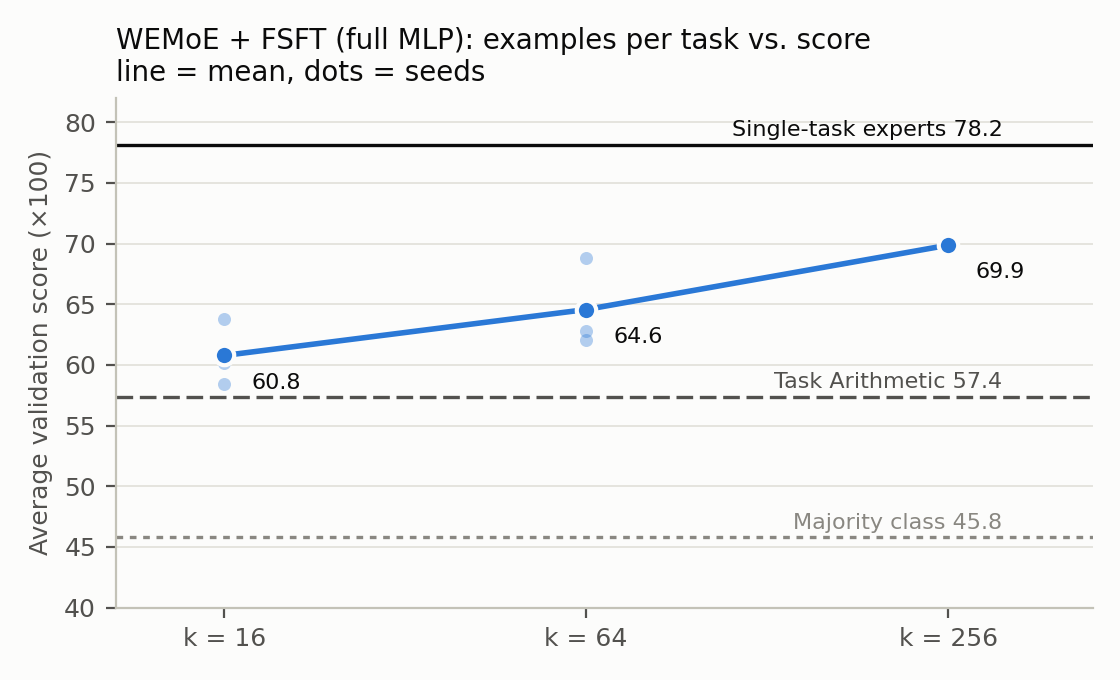
\includegraphics[width=.4\linewidth]{k_sweep.png}
  \caption{Average validation score of full-MLP WEMoE against the few-shot budget. The line shows the mean, and the dots show the seeds.}
  \label{fig:k-sweep}
\end{figure}

\section{Routing Behaviour}
\label{sec:routing}

Figure~\ref{fig:routing} shows the mean router values per layer and input task for one trained model. Many values lie far from their initial value of about $\lambda$, and both signs occur, which a convex mixture could not express. The panels look broadly alike, so much of the pattern is shared across input tasks, although they also differ in places, which shows that routing depends in part on the input. In this model, the column of the RTE expert is negative in the last two layers for every input type.

\begin{figure}[htbp]
  \centering
  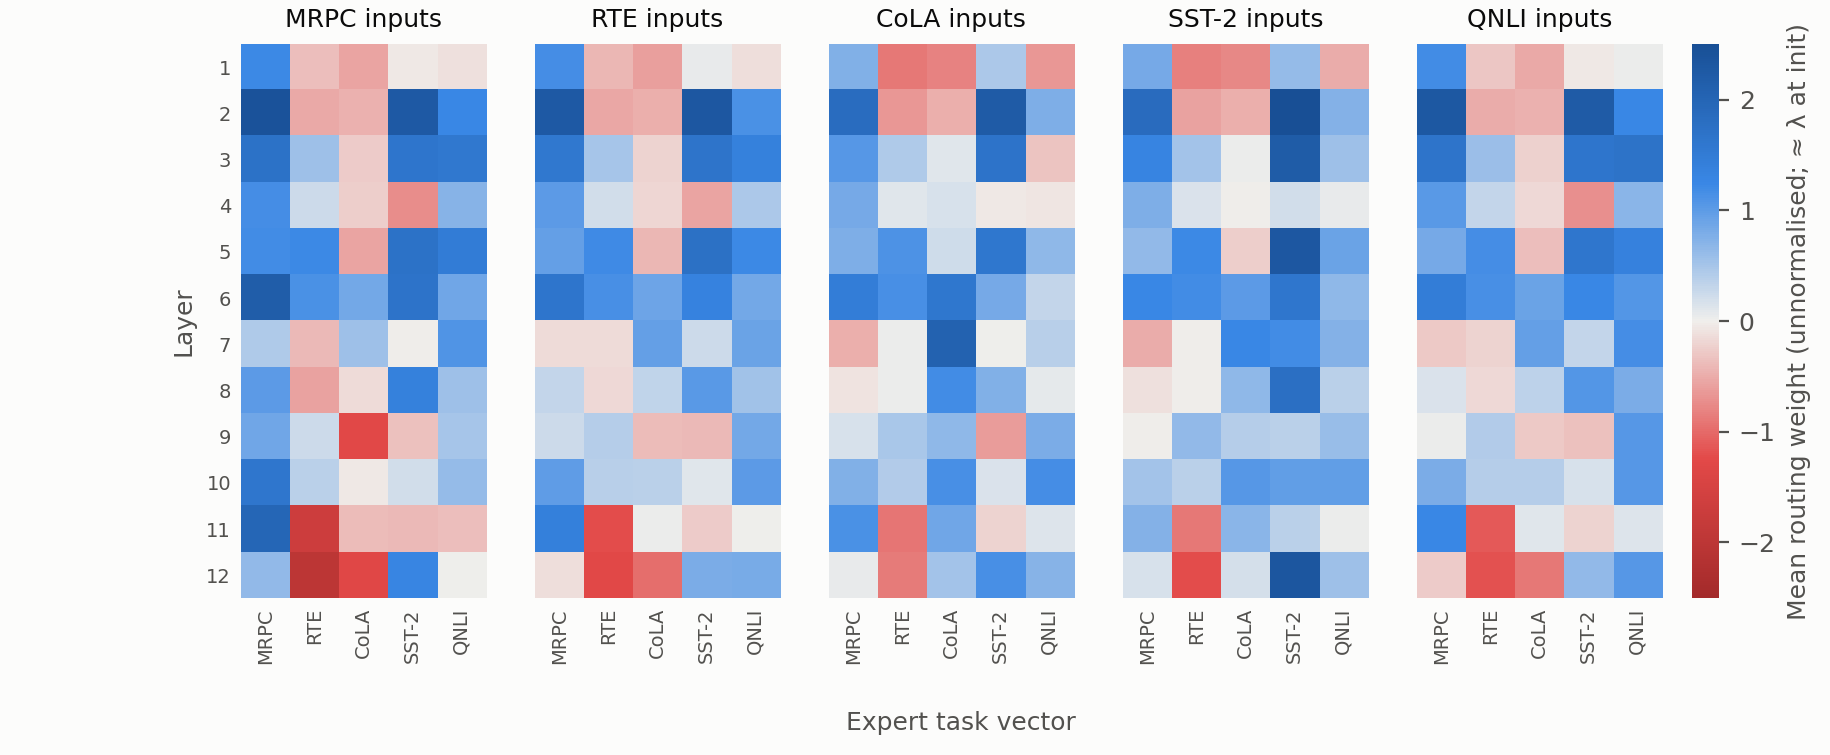
\includegraphics[width=.6\linewidth]{routing_clean.png}
  \caption{Mean router values per layer and input task (full MLP, $k=256$, seed 0). Blue adds and red subtracts a task vector.}
  \label{fig:routing}
\end{figure}

We quantified this pattern from the router values of every validation example. For seed 0, individual values range from $-3.0$ to $4.4$, and the per-layer sum of the values averaged over all examples reaches 5.8, against 1.5 at initialisation. The mean routing matrices of different input tasks correlate at 0.82 on average (0.84 for seeds 1 and 2), while the input task explains about 58\% of the routing variance (60\% for seeds 1 and 2). Table~\ref{tab:own} shows that most tasks up-weight their own expert, with RTE as the exception.

The RTE expert behaves differently across scopes, and one seed is not enough to read this difference. Its value on RTE inputs at layer 12 is negative under full-MLP upscaling on all three seeds ($-1.28$, $-0.65$, $-0.76$) and positive under intermediate-only upscaling ($2.04$, $1.16$, $1.53$). Its value averaged over layers is less stable: under intermediate-only upscaling it is 0.96, 0.27 and 0.31, while RTE accuracy stays between 58.1 and 59.9, so this average does not explain the RTE result. This evidence shows association only and does not establish why RTE fails.

\begin{table}[htbp]
  \centering\tablestyle
  \caption{Mean router value of a task's own expert, averaged over layers (full MLP, $k=256$, seed 0).}
  \label{tab:own}
  \begin{tabular}{l c c c c c}
    \toprule
    & MRPC & SST-2 & QNLI & CoLA & RTE\\
    \midrule
    On its own inputs & 1.37 & 1.37 & 0.94 & 0.61 & 0.01\\
    On other tasks' inputs & 0.77 & 0.67 & 0.56 & $-0.02$ & $-0.01$\\
    \bottomrule
  \end{tabular}
\end{table}

\section{Storage, Parameter Count and Inference Latency}
\label{sec:efficiency}

Table~\ref{tab:storage} breaks down the stored parameters, which match Equation~\eqref{eq:storage} and are measured on the built models. Task vectors dominate, at 283.3M of the 400.0M parameters of the full-MLP model.

\begin{table}[htbp]
  \centering\tablestyle
  \caption{Stored parameters (millions) by component, and total size at 32-bit precision.}
  \label{tab:storage}
  \setlength{\tabcolsep}{4pt}\begin{tabular}{l r r r r r r r r}
    \toprule
    Deployment & Static & Base MLP & Task vectors & Routers & Heads & Total & GiB & vs.\ 5 models\\
    \midrule
    5 single-task models & -- & -- & -- & -- & -- & 547.4 & 2.04 & 100.0\%\\
    Task Arithmetic & -- & -- & -- & -- & -- & 109.5 & 0.41 & 20.0\%\\
    WEMoE, full MLP & 52.8 & 56.7 & 283.3 & 7.13 & 0.008 & 400.0 & 1.49 & 73.1\%\\
    WEMoE, intermediate-only & 81.1 & 28.3 & 141.7 & 7.13 & 0.008 & 258.4 & 0.96 & 47.2\%\\
    \bottomrule
  \end{tabular}
\end{table}

Table~\ref{tab:latency} reports latency on one T4 GPU, with random token ids of length 128, mixed precision and the MRPC head, as the mean of 10 forward passes after 3 warm-up passes. The single-task row times one expert, because each input would go to its own expert by task identifier. Batch-1 figures are rough: they differed by up to 27\% between two measurement runs (24.05 ms and 18.90 ms for the intermediate-only model), while batch-32 times agreed within about 5\%. At batch size 32, the full-MLP model is about 4.5 times slower than one BERT and the intermediate-only model about 2.9 times, and the full-MLP model needs about 2.8 times the peak GPU memory.

\begin{table}[htbp]
  \centering\tablestyle
  \caption{Inference latency and peak GPU memory on one T4, from the final measurement run. $^{*}$Times one expert.}
  \label{tab:latency}
  \begin{tabular}{l c c c c}
    \toprule
    & \multicolumn{2}{c}{Batch 1} & \multicolumn{2}{c}{Batch 32}\\
    Deployment & ms/example & Peak MB & ms/example & Peak MB\\
    \midrule
    Single-task BERT$^{*}$ & 11.64 & 614 & 1.61 & 704\\
    Task Arithmetic & 12.67 & 435 & 1.63 & 519\\
    WEMoE, full MLP & 27.83 & 1615 & 7.31 & 1987\\
    WEMoE, intermediate-only & 18.90 & 1061 & 4.69 & 1387\\
    \bottomrule
  \end{tabular}
\end{table}
